% ================================================
% =              STATE OF THE ART                =
% ================================================ 

% Actualmente, la industria de la automoción está impulsando el desarrollo de los \aclink{ADS} con la promesa de reducir los accidentes en carretera y minimizar los costes tanto humanos como económicos que estos suponen \cite{survey_AutomatedDriving1}. Sin embargo, a pesar de que la conducción automatizada haya incrementado recientemente la atención de la industria por el auge del DeepLearning y la visión por ordenador, lo cierto es que lleva presente más de 20 años.

Currently, the automotive industry is driving the development of \aclink{ADS} with the promise of reducing road accidents and minimizing both the human and economic costs associated with them \cite{survey_AutomatedDriving1}. However, although automated driving has recently gained increased attention from the industry due to the rise of Deep Learning and computer vision, it has actually been present for more than 20 years.

% Algunas de las primeras competiciones de conducción automatizada, como los DARPA Challenges en 2003 y 2005 o el Grand DARPA Urban challenge de 2007, impulsaron enormemente el desarrollo de los \aclink{ADS}, atrayendo la atención tanto de empresas tecnológicas como del sector automotriz \cite{survey_AutomatedDriving2}. Este avance ha sido acompañado por la definición de buenas prácticas y procesos de estandarización para garantizar la seguridad y fiabilidad de los \aclink{ADS}. En este contexto, la \aclink{SAE} ha establecido una escala progresiva de automatización, desde el nivel 0 (sin automatización) hasta el nivel 5 (automatización total), definiendo el grado de intervención del conductor en cada etapa \cite{AD_Technical_Standards}. 

Some of the earliest automated driving competitions, such as the DARPA Challenges in 2003 and 2005 or the Grand DARPA Urban Challenge in 2007, significantly boosted the development of \aclink{ADS}, attracting the attention of both technology companies and the automotive sector \cite{survey_AutomatedDriving2}. This progress has been accompanied by the establishment of best practices and standardization processes to ensure the safety and reliability of \aclink{ADS}. In this context, the \aclink{SAE} has defined a progressive scale of automation, ranging from Level 0 (no automation) to Level 5 (full automation), specifying the degree of driver intervention required at each stage \cite{AD_Technical_Standards}.

% Hoy en día, la mayoría de los vehículos incorporan sistemas avanzados de asistencia a la conducción \aclink{ADAS}, que operan en los niveles \aclink{SAE} 2 y 3. No obstante, ya existen \aclink{ADS} de nivel 4, como los desarrollados por Waymo y Cruise para robotaxis, o los autobuses autónomos desplegados en algunas ciudades, cuyos sistemas están diseñados para gestionar el fallback de manera autónoma, sin necesidad de intervención humana \cite{fallback_strategy}.

Today, most vehicles incorporate Advanced Driver Assistance Systems (\aclink{ADAS}), which operate at \aclink{SAE} Levels 2 and 3. However, Level 4 \aclink{ADS} already exist, such as those developed by Waymo and Cruise for robotaxis, as well as autonomous buses deployed in some cities. These systems are designed to manage fallback autonomously, without the need for human intervention \cite{fallback_strategy}.

% Este desarrollo ha llevado a la creación de distintas estrategias y arquitecturas para los \aclink{ADS}. En los últimos años, ha habido grandes avances en soluciones \mbox{End-to-End}, que combinan técnicas de aprendizaje profundo y aprendizaje por refuerzo para obtener las acciones de control del vehículo partiendo diréctamente de los datos de los sensores \cite{end_to_end_driving}. Sin embargo, la mayoría de los enfoques optan por soluciones modulares más tradicionales, que dividen el problema de la conducción automatizada en \mbox{sub-tareas} específicas, integrando soluciones de campos como la robótica, visión por ordenador, deep learning y control automático.

This development has led to the creation of various strategies and architectures for \aclink{ADS}. In recent years, significant progress has been made in \mbox{End-to-End} solutions, which combine deep learning and reinforcement learning techniques to derive vehicle control actions directly from sensor data \cite{end_to_end_driving}. However, most approaches favor more traditional modular solutions, which divide the automated driving problem into specific \mbox{sub-tasks}, integrating solutions from fields such as robotics, computer vision, deep learning, and automatic control.

% En el contexto de las arquitecturas modulares, la adopción de buenas prácticas ha facilitado la categorización de estas \mbox{sub-tareas} en tres grupos principales \cite{machines5010006}\cite{functional_architectures}: 
% \begin{itemize}
%     \item Percepción, que se refiere a la capacidad del sistema autónomo para recolectar información del entorno y extraer conocimiento relevante, como la ubicación de obstáculos, señales de tráfico y la localización del vehículo.
%     \item Planificación del comportamiento, que consiste en tomar decisiones para alcanzar los objetivos del vehículo, como llegar de un punto a otro evitando obstáculos y optimizando la trayectoria.
%     \item Ejecución de movimientos, que se refiere a la capacidad del vehículo para ejecutar las acciones planificadas por el sistema, controlando la dirección, velocidad y maniobras necesarias.
% \end{itemize}
% Además, estas \mbox{sub-tareas} interactúan entre sí, con el hardware del vehículo y con sistemas de comunicación como \aclink{V2I} o \aclink{V2X} en el caso de los vehículos conectados.

In the context of modular architectures, the adoption of best practices has facilitated the categorization of these \mbox{sub-tasks} into three main groups \cite{machines5010006}\cite{functional_architectures}:  

\begin{itemize}  
    \item \textbf{Perception}, which refers to the autonomous system's ability to gather environmental information and extract relevant knowledge, such as the location of obstacles, traffic signs, and the vehicle’s position.  
    \item \textbf{Behavior planning}, which involves making decisions to achieve the vehicle's objectives, such as reaching a destination while avoiding obstacles and optimizing the trajectory.  
    \item \textbf{Motion execution}, which pertains to the vehicle’s ability to carry out the planned actions by controlling steering, speed, and necessary maneuvers.  
\end{itemize}

Furthermore, these \mbox{sub-tasks} interact with each other, with the vehicle's hardware, and with communication systems such as \aclink{V2I} or \aclink{V2X} in the case of connected vehicles.

\begin{figure}[H]
    \centering
    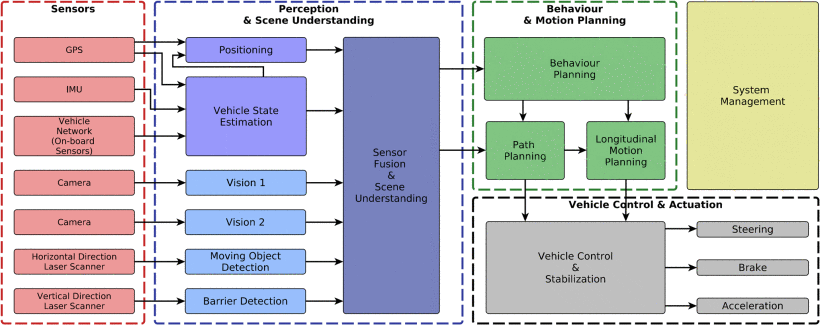
\includegraphics[width=\linewidth]{images/sota/ADS_information_flow.png}
    \label{sota_ads_information_flow}
    \caption{Arquitectura modular de un ADS. TEMPORAL!!!}
\end{figure}

% En este tipo de arquitecturas, un error en una \mbox{sub-tarea} puede propagarse y afectar el desempeño de otras, comprometiendo así el funcionamiento del sistema. Esto es especialmente crítico en el módulo de percepción, ya que la calidad de la información obtenida impacta directamente en tareas posteriores como la localización, el mapeo y la planificación. Por ello, garantizar sistemas de percepción robustos es fundamental para el rendimiento y la seguridad de los \aclink{ADS}.

In these types of architectures, an error in one \mbox{sub-task} can propagate and affect the performance of others, potentially compromising the overall system functionality. This is particularly critical in the perception module, as the quality of the obtained information directly impacts subsequent tasks such as localization, mapping, and planning. Therefore, ensuring robust perception systems is essential for the performance and safety of \aclink{ADS}.

% Dos de las tareas principales de los sistemas de percepción en los \aclink{ADS} son la detección 3D de objetos y la segmentación en \aclink{BEV}. La detección 3D de objetos es una de las tareas más relevantes y comúnmente se basa en nubes de puntos obtenidas mediante sensores LiDAR. En ausencia de LiDAR, una alternativa es la detección 3D multi-cámara, que busca predecir cajas delimitadoras 3D en un sistema de coordenadas \aclink{BEV} utilizando únicamente imágenes monoculares. Por otro lado, la segmentación en \aclink{BEV} tiene como objetivo realizar una segmentación semántica del entorno, identificando áreas transitables y delimitaciones de carril en el marco de referencia del vehículo. A diferencia de la detección de objetos, la segmentación en \aclink{BEV} permite una predicción densa de clases estáticas del entorno, lo que resulta clave para la construcción de mapas locales, estimación del comportamiento de agentes y downstream tasks como la planificación del comportamiento del \aclink{ADS}. \hl{Añadir referencias.}

Two of the main perception tasks in \aclink{ADS} are 3D object detection and \aclink{BEV} segmentation. 3D object detection is one of the most crucial tasks and is commonly based on point clouds obtained from LiDAR sensors. In the absence of LiDAR, an alternative is multi-camera 3D detection, which aims to predict 3D bounding boxes in a \aclink{BEV} coordinate system using only monocular images.

On the other hand, \aclink{BEV} segmentation focuses on performing semantic segmentation of the environment, identifying drivable areas and lane boundaries in the vehicle's reference frame. Unlike object detection, \aclink{BEV} segmentation enables dense prediction of static environment classes, which is essential for local map construction, agent behavior estimation, and downstream tasks such as behavior planning in \aclink{ADS}. \hl{Add references.}

This thesis is developed within the context of \aclink{BEV} semantic segmentation \hl{...}.

\subsection{Semantic segmentation}

\subsection{BEV semantic segmentation}
Traditional methods \cite{3d_traffic_scene_understanding} estimate local \aclink{BEV} maps using camera inputs under the flat-ground assumption applying \aclink{IPM}. However, these methods require accurate camera parameters which has led to research focusing on camera parameter estimation for \aclink{BEV} transformation \cite{BEV_params_estimation1} \cite{BEV_params_estimation2}. Another key challenge in \aclink{BEV} map generation is handling object occupancy and occlusion. \aclink{ADS} must be aware of objects dimensions and should account for uncertainty in vehicular scenes. However, estimating vehicle occupancy is non-trivial as the necessary perspective views of objects are often unavailable. In this context, there are many reseachs that addresses the local semantic map estimation with different approaches.

Cam2BEV \cite{Cam2BEV} applies \aclink{IPM} to transform multi-camera segmented input images into the \aclink{BEV} domain which is feeded into the model to refine the \aclink{BEV} representation. To handle occlusions, Cam2BEV introduces an additional semantic class that explicitly marks occluded areas from all vehicle-mounted cameras. As the input of the model are already segmented images, an extra \aclink{CNN} was employed to test the method in real-world data.  

HDMapNet \cite{HDMapNet} generates high-definition semantic maps from multi-camera input by employing a feature projection module that transforms image features into \aclink{BEV} space. The model first extracts image features and transforms them into the camera coordinate system with a shared \aclink{MLP} backbone, and then projects them into \aclink{BEV} using camera extrinsics. Finally a semantic segmentation decoder is used.

PYVA \cite{PYVA} introduces a cross-view transformer that projects features from the front-view domain to the \aclink{BEV} domain. While similar to HDMapNet, PYVA differs in that it does not rely on camera parameters in the second transformation stage as the model is cappable of learning this transformation. Different to other methods, this work uses a GAN-based framework to manage occluions by estimating the vehicle's top view masks. However, this method is not suitable for multi-camera fusion.

Other approaches propose different architectures for \aclink{BEV} semantic segmentation. VPN \cite{view_parsing_network} introduces a two-layer \aclink{MLP} module for multi-camera feature fusion, followed by a decoder for semantic segmentation in indoor scenes. LSS \cite{lift_splat_shoot} proposes a unified framework that lifts 2D images into a 3D space by learning an implicit depth distribution and shows that their method is suitable for end-to-end motion plannig. M²BEV \cite{m2bev} transforms 2D image features into 3D voxels along projection rays and obtains an efficient \aclink{BEV} representation which supports multiple end tasks such as semantic segmentation or object 3D detection.

MonoLayout \cite{mono_layout} tackles occlusion estimation by employing a standard encoder-decoder framework combined with adversarial training, making it suittable for predicting amodal layouts of the driving scene. BEVFormer \cite{BEVFormer} similarly enhances occlusion reasoning by leveraging attention mechanisms to fuse multi-view spatial-temporal features from historical \aclink{BEV} maps.

There are also methods that combines information form multiple sensor such as FishingNet \cite{fishingnet} which extends VPN to use multiple sensors, or HDMapNet which is also cappable of using \aclink{LiDAR} sensors.  


In summary, existing approaches to local \aclink{BEV} map estimation typically follow one of two strategies: 
\begin{enumerate}
    \item Performing early-stage segmentation on input images before refining the \aclink{BEV} representation.
    \item Learning to embed image features into \aclink{BEV} space before passing them through a semantic segmentation decoder.
\end{enumerate}
However, to the best of our knowledge, no previous work directly trains a model on already-reprojected \aclink{BEV} images.

Instead of applying semantic segmentation before transforming images into \aclink{BEV} space, we study whether training a segmentation model directly on top-view images improves the representation of planar elements compared to the traditional segmentation-first-then-IPM approach. Furthermore, we treat occupancy and occlusion mask generation as a post-processing step applied to \aclink{BEV} semantic segmentation, where 3D object detection is performed. This is integrated into a pre-annotation pipeline for vehicle scenes, contributing to advancements in monocular 3D object detection. 

